\documentclass[12pt,a4paper,twoside, openright]{scrartcl} 
\usepackage[scaled]{helvet}
\usepackage[italian]{babel}
\usepackage[utf8]{inputenc}
\usepackage[T1]{fontenc}
\usepackage{fancyhdr}
\usepackage{lastpage}
%\usepackage{ifthen}
\usepackage{amsmath,amsfonts,amsthm}
\usepackage{sfmath}
\usepackage{sectsty}
\usepackage{listings}
\lstset{language=Matlab,frame=single,numbers=left}
\usepackage{graphicx}
\usepackage{float}
\usepackage{amsthm}
\usepackage{caption}
\usepackage{subfig}
\addtokomafont{caption}{\small}
\setkomafont{captionlabel}{\normalfont\bfseries}
\let\oldtabular\tabular
\renewcommand{\tabular}{\sffamily\oldtabular}
%\KOMAoptions{abstract=true}
\renewcommand\familydefault{\sfdefault}
\renewcommand{\arraystretch}{1.1}
\newcommand{\horrule}[1]{\rule{\linewidth}{#1}}
\setlength{\textheight}{230mm}
\allsectionsfont{\centering \normalfont\scshape}
\let\tmp\oddsidemargin
\let\oddsidemargin\evensidemargin
\let\evensidemargin\tmp
\reversemarginpar
\setlength\parindent{0pt}


\graphicspath{{Sorgenti/}}
\newcommand{\thetap}{\dot{\theta}}
\newcommand{\thetapp}{\ddot{\theta}}
\newcommand{\Xu}{X_1}
\newcommand{\Xup}{\dot{X_1}}
\newcommand{\xu}{x_1}
\newcommand{\xd}{x_2}
\newcommand{\xt}{x_3}
\newcommand{\xup}{\dot{x}_1}
\newcommand{\xdp}{\dot{x}_2}
\newcommand{\xtp}{\dot{x}_3}
\newcommand{\yu}{y_1}
\newcommand{\yd}{y_2}
\newcommand{\yt}{y_3}

\fancypagestyle{plain}
{
	\renewcommand{\headrulewidth}{0pt}%
	\renewcommand{\footrulewidth}{0.5pt}
	\fancyhf{}%
	\fancyfoot[R]{\emph{\footnotesize Page \thepage\ of \pageref{LastPage}}}%
	\fancyfoot[C]{\emph{\footnotesize Leonardo Soccio}\\ \emph{\footnotesize 0251992}}%
}
%\author{Leonardo Soccio}
\title{Analisi Fisica del progetto}
\date{\vspace{-5ex}}
%\date{} 

\begin{document}
	\pagestyle{plain}
	\maketitle
	Il sistema può essere ricondotto a un asta vincolata nel punto  $O$ e a un disco vincolato in $D$ che viene messo in moto da un motore.\\ 
	Lo scopo dell'analisi è capire come varia l'angolo $\theta$ con la verticale in modo tale da poterlo controllare controllando il motore che muove il disco.
\section{Rappresentazione del sistema}
		\begin{figure}[H]
			\begin{center}
				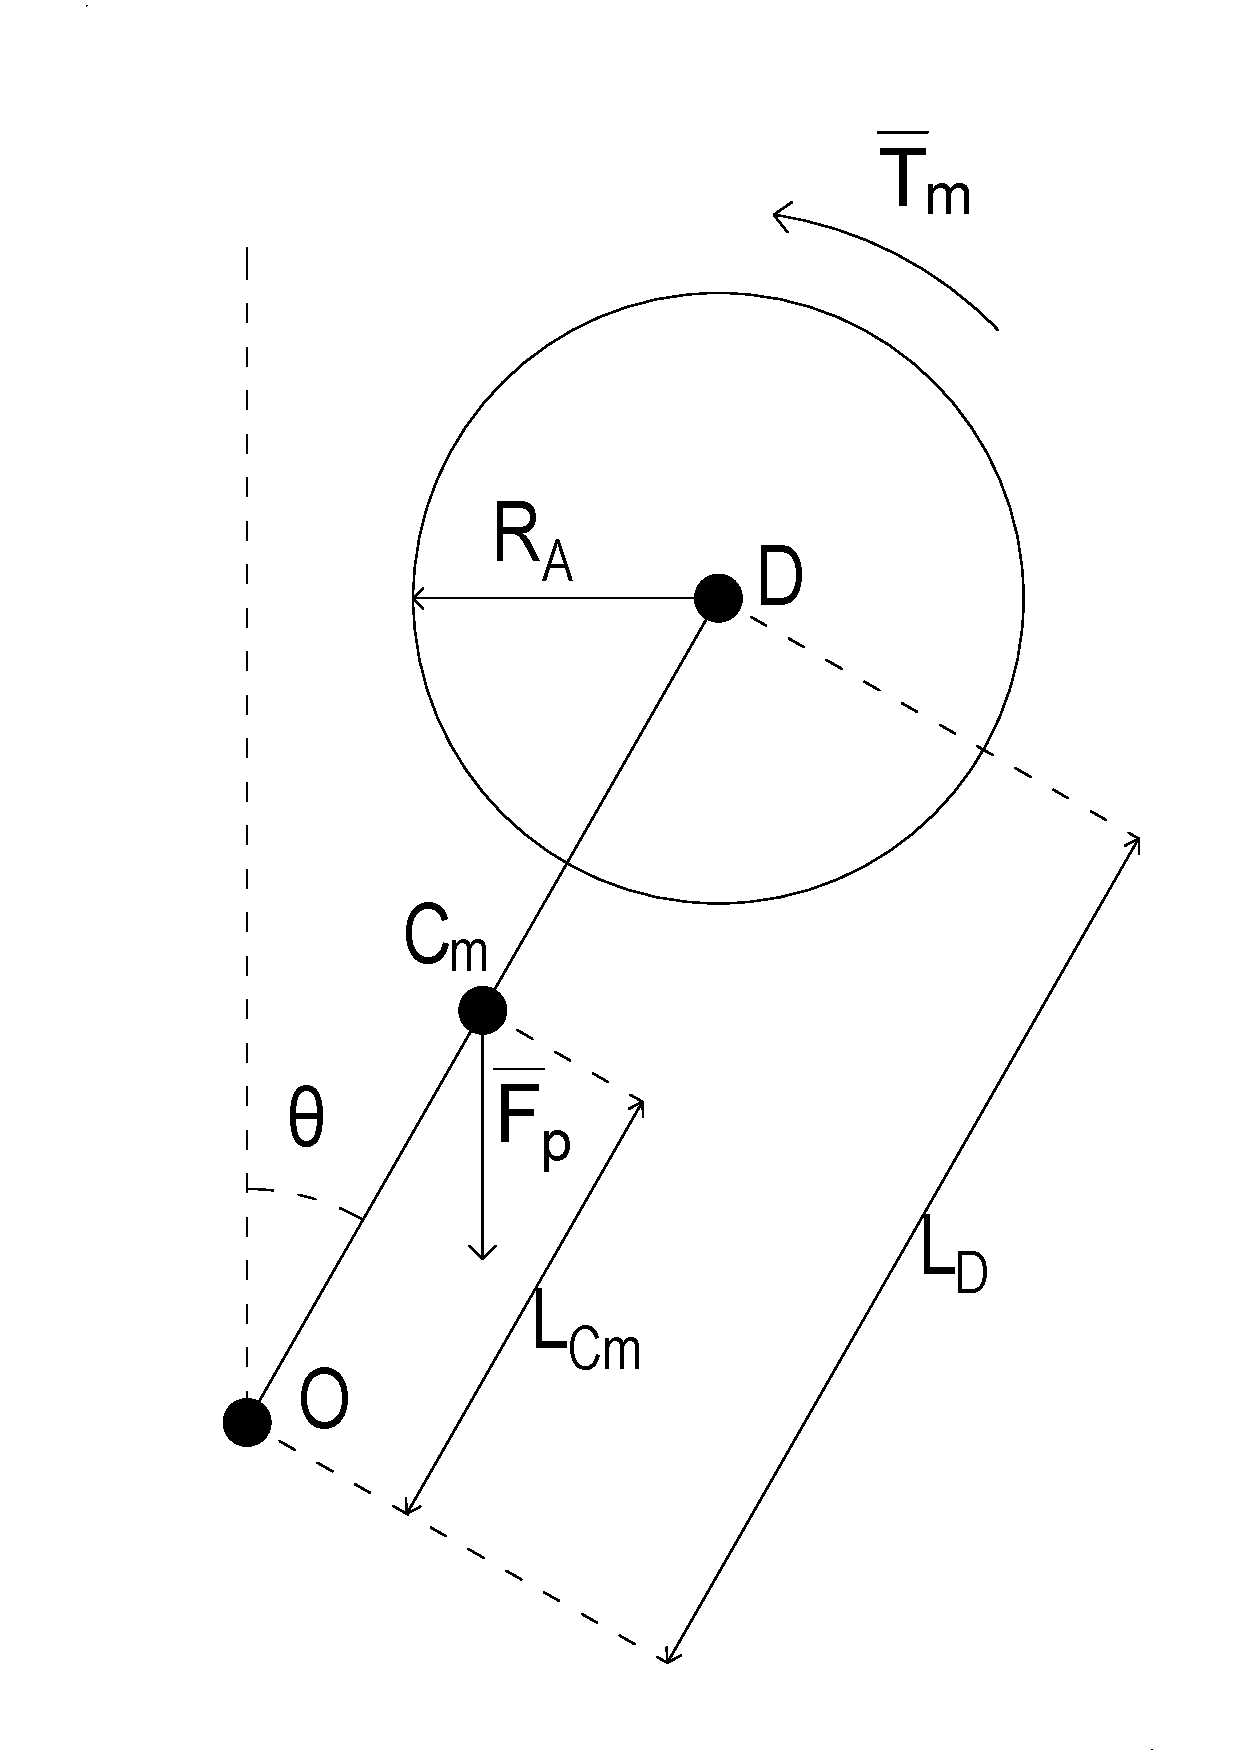
\includegraphics[height=8cm]{Sorgenti/Figura1.pdf}
			\end{center}
				%\caption{Schema del pendolo inverso}
			\label{fig:struttura}
		\end{figure}
	Le caratteristiche del sistema sono:
	\begin{itemize}
		\item $O$ è il punto in cui il sistema è vincolato;
		\item $\theta$ è l'angolo di inclinazione rispetto la verticale dell'asta;
		\item $C_m$ è il centro di massa dell'intero sistema, considerando anche la ruota;
		\item $L_{C_m}$ è la distanza del centro di massa $C_m$ dal polo $O$; 
		\item $D$ è il punto in cui è vincolata la ruota e il motore(non rappresentato);
		\item $L_D$ è la distanza del punto $D$ dal polo $O$; 
		\item $\overline{F}_p$ è la forza peso totale agente sul sistema, considerata applicata nel centro di massa;
		\item $ \overline{\tau}_m$ è la coppia che il motore fornisce al sistema;
		\item $I_t$ è l'inerzia totale del sistema rispetto il polo $O$;
		\item $I_d$ è l'inerzia del disco rispetto il punto $D$;
	\end{itemize}
	Per l'analisi considererò trascurabili tutti gli attriti e considerero la coppia del motore linearmente legata alla tensione.\\
	Per la seconda equazione cardinale della meccanica si avrà che:
	\begin{equation}
		\label{eqn:1}
		I_t\thetapp=F_p L_{C_m}\sin(\theta)- \tau_m
	\end{equation}
	per chiarezza nell'esposizione pongo $F_p L_{C_m}=K_{mgl}$ in quanto valore costante.
	Inoltre:
	\begin{equation}
		\label{eqn:2} 
	 	\tau_m =I_d \dot{w}_{inerziale}
	 \end{equation}
	Dove:\\
	 $\dot{w}_{inerziale}$ è la velocità angolare assoluta del disco;
	Infine dai moti relativi vale che:
	\begin{equation}
		\label{eqn:4}
		w_{inerziale}=\thetap+w_R 
	\end{equation}
	e sostituendo nella \ref{eqn:2}
	\begin{equation}
		\label{eqn:5}
		\tau_m =I_d (\dot{w}_{R}+\thetapp)
	\end {equation}
	In prima battuta per simulare il sistema si è preferito usare la coppia effettiva sul disco come grandezza di controllo, di conseguenza le equazioni sono state riscritte per l'utilizzo:
\begin{align}
	\thetapp&=\frac{K_{mgl}}{I_t}\sin(\theta) -\frac{\tau_m}{I_t} \label{eqn:6}\\
	\dot{w}_R&=-\thetapp + \frac{\tau_m}{I_d} \label{eqn:7}
\end{align}
	Per poter computare il sistema si è attuato un cambio di variabile ponendo:
\begin{align}
\xu&=\thetap\qquad	  \xup=\thetapp  \label{eqn:8}\\
\xd&=\theta 	\qquad	  \xdp=\thetap \label{eqn:9}\\
u&=\tau_m \qquad \xt=w_R \label{eqn:10}
\end{align}
	date le seguenti sostituzioni il sistema diventa:
\begin{equation}
	\label{sis:1}
	\begin{cases}
		\xup=\frac{K_{mgl}}{I_t}\sin(\xd) -\frac{1}{I_t}u   \\
		\xdp=\xu\\
		\xtp=-\frac{K_{mgl}}{I_t}\sin(\xd) +\big(\frac{1}{I_t}+\frac{1}{I_d}\big)u 
	\end{cases}
\end{equation}
	definiamo quindi il vettore $\Xup$ :
\begin{equation}
	\label{eqn:11}
	\Xup =
	\begin{bmatrix}
		\xup \\
		\xdp \\
		\xtp
	\end{bmatrix}
	=
		\begin{bmatrix}
		\thetapp \\
		\thetap \\
		\dot{w}_R
	\end{bmatrix}
\end{equation}
Infine definiamo il vettore stato $Y$ come:
\begin{equation}
	\label{eqn:12}
	Y=
	\begin{bmatrix}
		\yu \\
		\yd \\
		\yt
	\end{bmatrix}
	=
	\begin{bmatrix}
		\xu \\
		\xd \\
		\xt
	\end{bmatrix}
\end{equation}	

\end{document}
